\chapter{The \LHC and the \CMS experiment}
\label{chap:detector}

The purpose of this chapter is to introduce the \CMS experiment~\cite{Chatrchyan:2008aa} and the \LHC~\cite{1748-0221-3-08-S08001}. Without both of these apparatus the analyses performed for this thesis would, of course, not have been possible. In \SectionRef{sec:lhc} an overview of the \LHC and the chain of accelerators which feed into it will be given. This will then be followed in \SectionRef{sec:CMSInDetail} by a description of the \CMS experiment focussing on the aspects most relevant to the search for invisibly decaying Higgs bosons.

\section{The \LHC}
\label{sec:lhc}
The \LHC is situated 100m underground in a tunnel formerly built for the LEP accelerator~\cite{lepdesign} at CERN near Geneva, Switzerland. It is a 27km storage ring which accelerates both protons and heavy ions and collides them at the highest centre of mass energies of any collider built to date. The work contained in this thesis uses data from proton-proton collisions. These protons are obtained by taking hydrogen gas and stripping its atoms of their electrons with an electric field. The first accelerator in the \LHC accelerator sequence, Linac 2, accelerates the protons to 50 \MeV. The protons are then accelerated to 1.4 \GeV~by the next accelerator, the \ac{PSB}, which is followed by the \ac{PS} where they reach 25 \GeV. The beam energy is then increased to 450 \GeV~in the \ac{SPS}. Finally, the protons are injected into the \LHC where, at time of writing, the maximum energy the beams have been accelerated to is 6.5 \TeV, close to the design maximum of 7 \TeV.

When fully filled the \LHC contains two counter-rotating beams which are formed of up to 2808 bunches spaced either 25 or 50 ns apart and each containing $\mathcal{O}(10^{11})$ protons. The two beams are kept travelling in a cirlce by 1232 superconducting dipole magnets and steered to four collision points around the \LHC. Detectors are situated at these collision points to observe the collisions, the main four being: ALICE~\cite{Aamodt:2008zz}, ATLAS~\cite{Aad:1129811}, CMS~\cite{Chatrchyan:2008aa} and LHCb~\cite{Alves:2008zz}. A schematic of the LHC accelerator chain and the detectors can be seen in \FigureRef{fig:lhclayout}.

\begin{figure}
  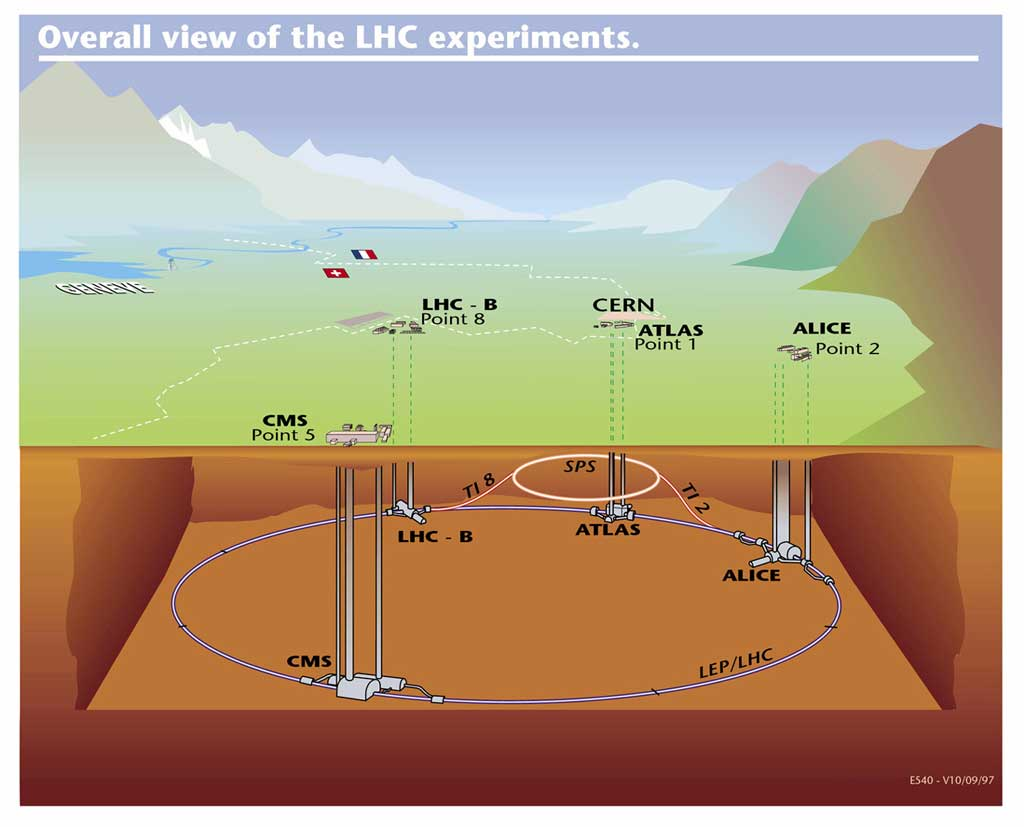
\includegraphics[width=\largefigwidth]{plots/detector/lhc_layout_sch.jpg}
  \caption{The layout of the LHC accelerator chain, showing the position of the four main detectors.}
  \label{fig:lhclayout}
\end{figure}

When studying a physical process occuring in particle collisions it is important to know how many times it will occur, this can be expressed as:
\begin{equation}
  N = \mathcal{L}\sigma,
\end{equation}
where $\mathcal{L}$, the integrated luminosity, depends only on the parameters of the collisions, and the cross-section depends only on the process. In order to observe rare (i.e. low cross-section) processes, such as those studied at the LHC, it is, necessary to use very high luminosity datasets. The integrated luminosity is obtained by integrating the instantaneous luminosity over time, so large luminosities can be obtained either by running the accelerator for a long time, or by operating at high instantaneous luminosity. For collisions at the LHC the instantaneous luminosity is given by:
\begin{equation}
  \mathcal{L}=\frac{k_{b}N_{b}^{2}f_{rev}\gamma}{4\pi\epsilon_{n}\beta}, \cite{Benedikt:823808}
\end{equation}
where $k_{b}$ is the number of bunches per beam, $N_{b}$ the number of protons per bunch, $f_{rev}$ the revolution frequency, $\epsilon_{n}$ the normalised transverse beam emittance, $\beta^{*}$ the beta-function at the interaction point and $\gamma$ the Lorentz factor. The design instantaneous luminosity of the LHC is $10^{34}\,\cm^{-2}\rm{s}^{-1}$ with 25ns bunch spacing.

The LHC started physics runs in 2010, during which it operated at a centre of mass energy of 7 \TeV~ and delivered an integrated luminosity of 44.2 \invpb ~to CMS. In 2011 the LHC also operated at 7 \TeV~ and delivered 6.1\invfb to CMS. The centre of mass energy was increased to 8 \TeV~ in 2012 and 23.3\invfb~of data were delivered to CMS. A summary of the luminosity delivered to CMS during the three runs can be seen in \FigureRef{fig:lumisummary}  %??Design and actual luminosity so far 
%??13 TeV lumi

\begin{figure}
  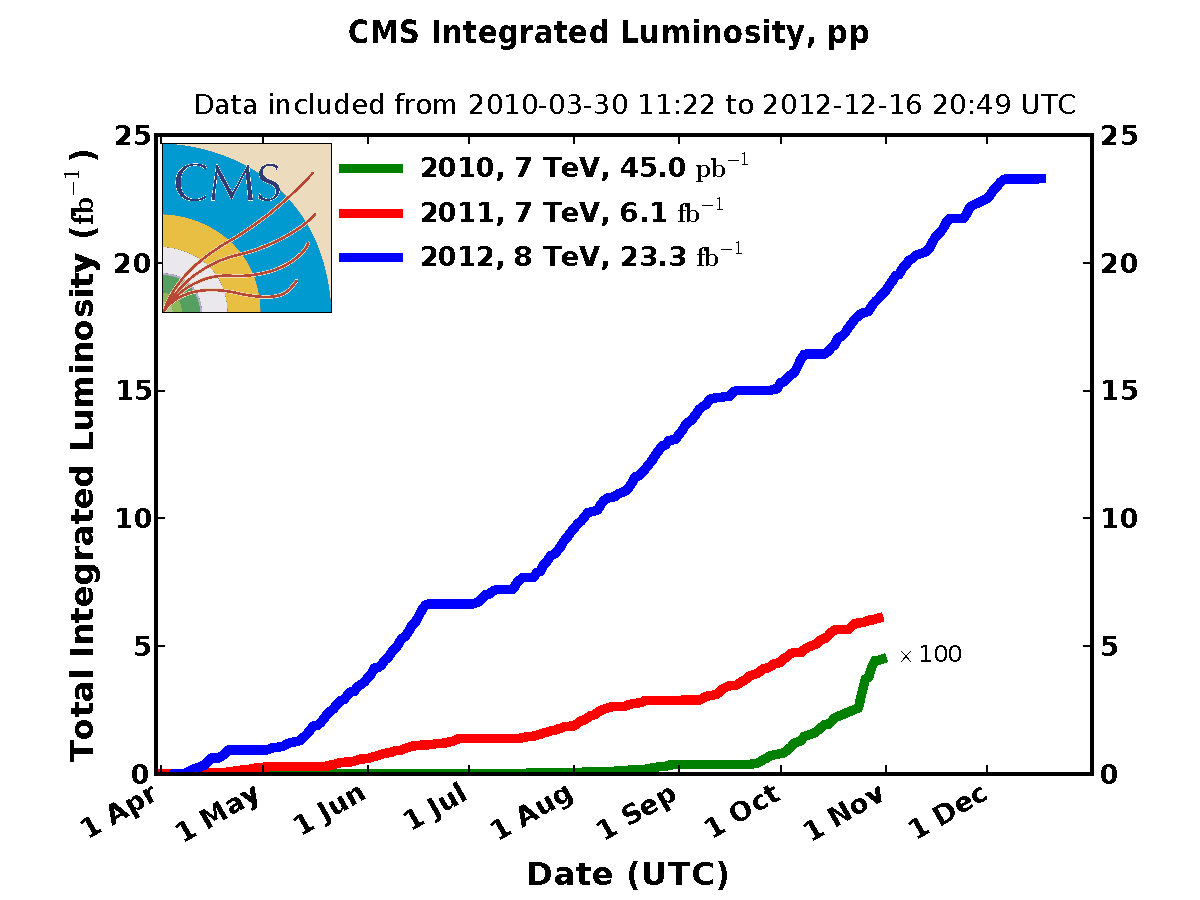
\includegraphics[width=1.2\largefigwidth]{plots/detector/int_lumi_cumulative_pp_2.pdf}
  \caption{A summary of the luminosity delivered to CMS during Run 1 of the LHC.\cite{CMSLumiPublic}}
  \label{fig:lumisummary}
\end{figure}
%??maybe figure for 13 TeV too

The cross-section for several processes is shown in \FigureRef{fig:xssummary} and it can be seen that the cross-section for VBF Higgs production is approximately 1.5 pb. Therefore, we expect approximately 30000 VBF produced Higgs bosons in the 2012 dataset. By contrast the vector boson production cross section is approximately 100 nb and the total cross-section for any process is orders of magnitude higher still. The separation of the relatively small number of signal events from the large background is a major challenge for the search for Higgs to invisible.

\begin{figure}
  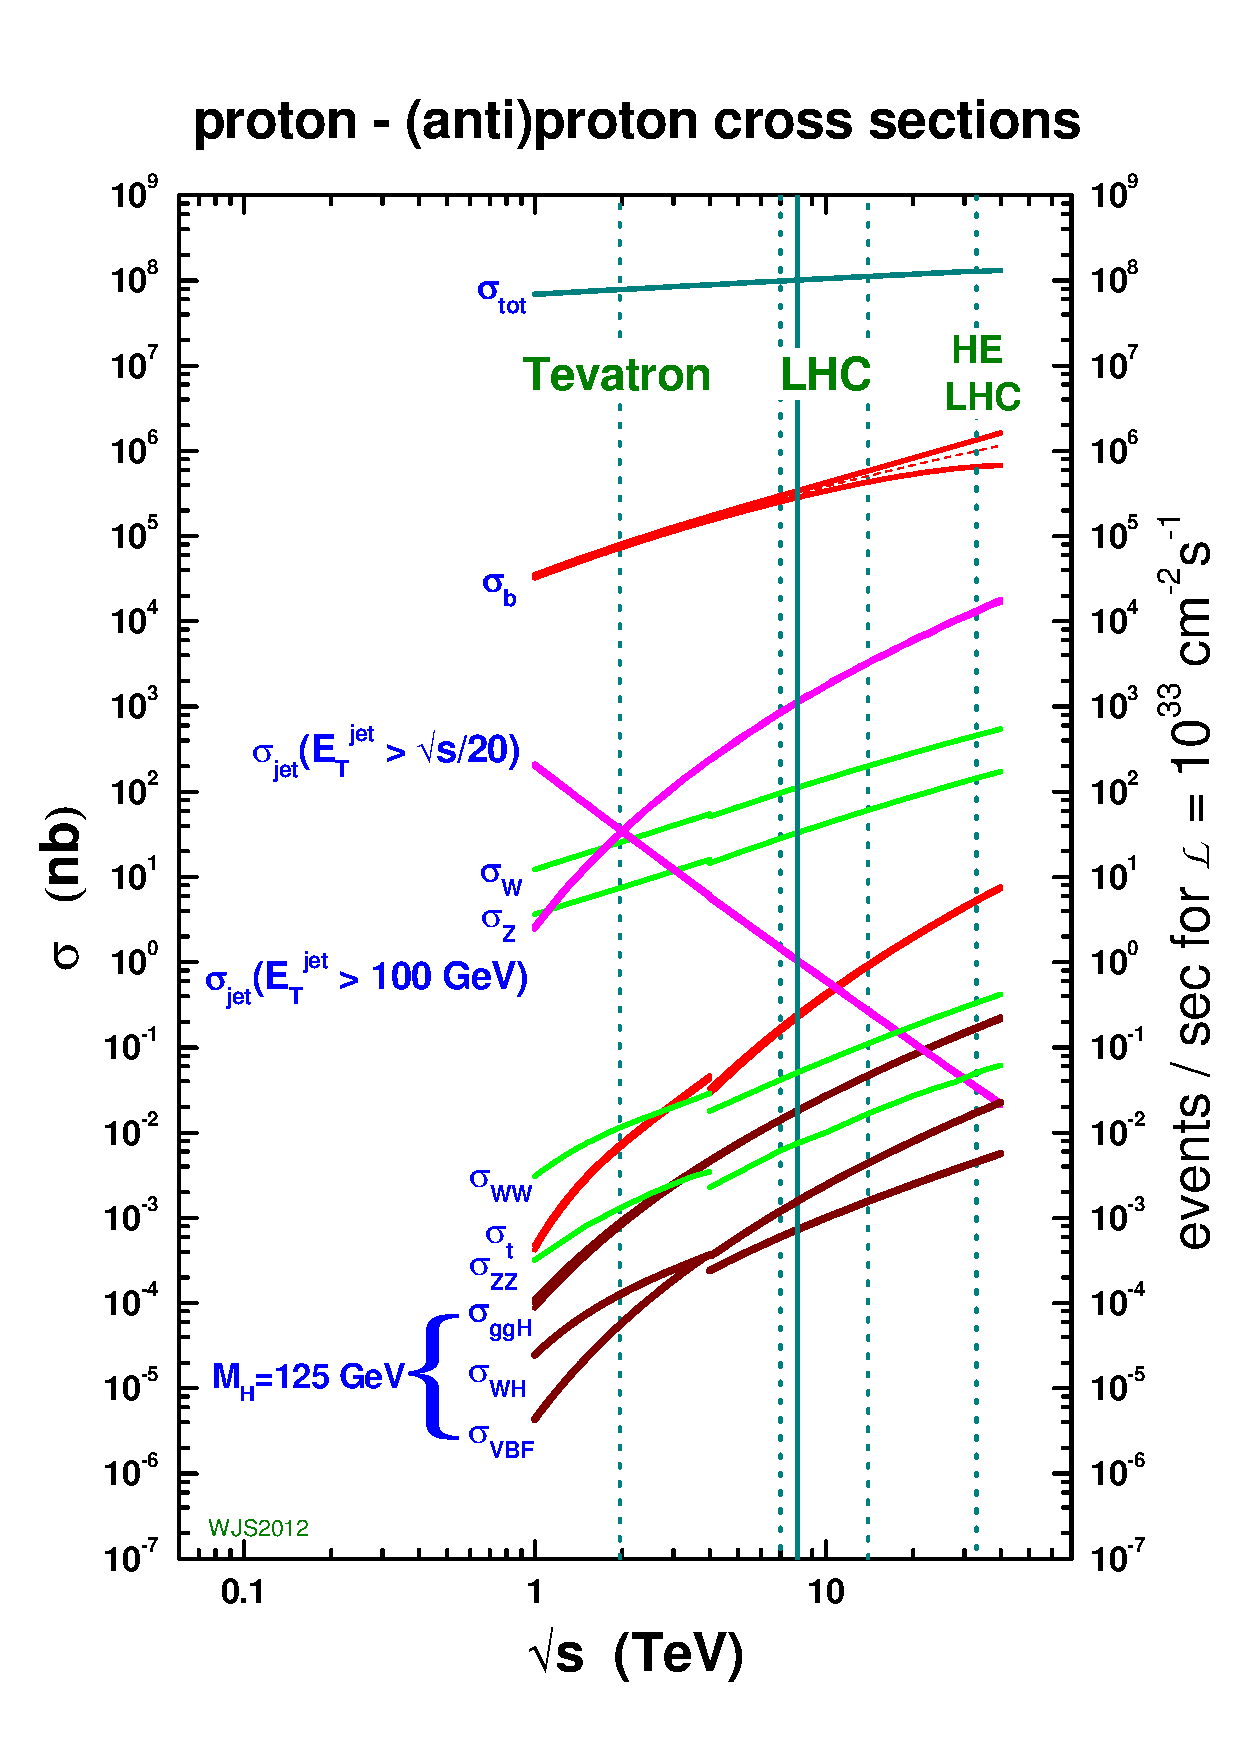
\includegraphics[width=1.2\largefigwidth]{plots/detector/crosssections2012HE_v4.pdf}
  \caption{Cross sections for several processes in collisions of protons with protons or anti-protons as a function of centre of mass energy. The energies that the LHC and Tevatron ran at are highlighted.\cite{Stirlingppxs}}
  \label{fig:xssummary}
\end{figure}

The large total cross-section combined with the high instantaneous luminosities that the LHC operates at leads to the probability for multiple proton-proton interactions per bunch crossing being high. The distribution of the number of interactions per bunch crossing can be seen in \FigureRef{fig:pusummary}. The additional interactions on top of the process of interest in a bunch crossing are called pile-up \ac{PU}.
%??Define an event

\begin{figure}
  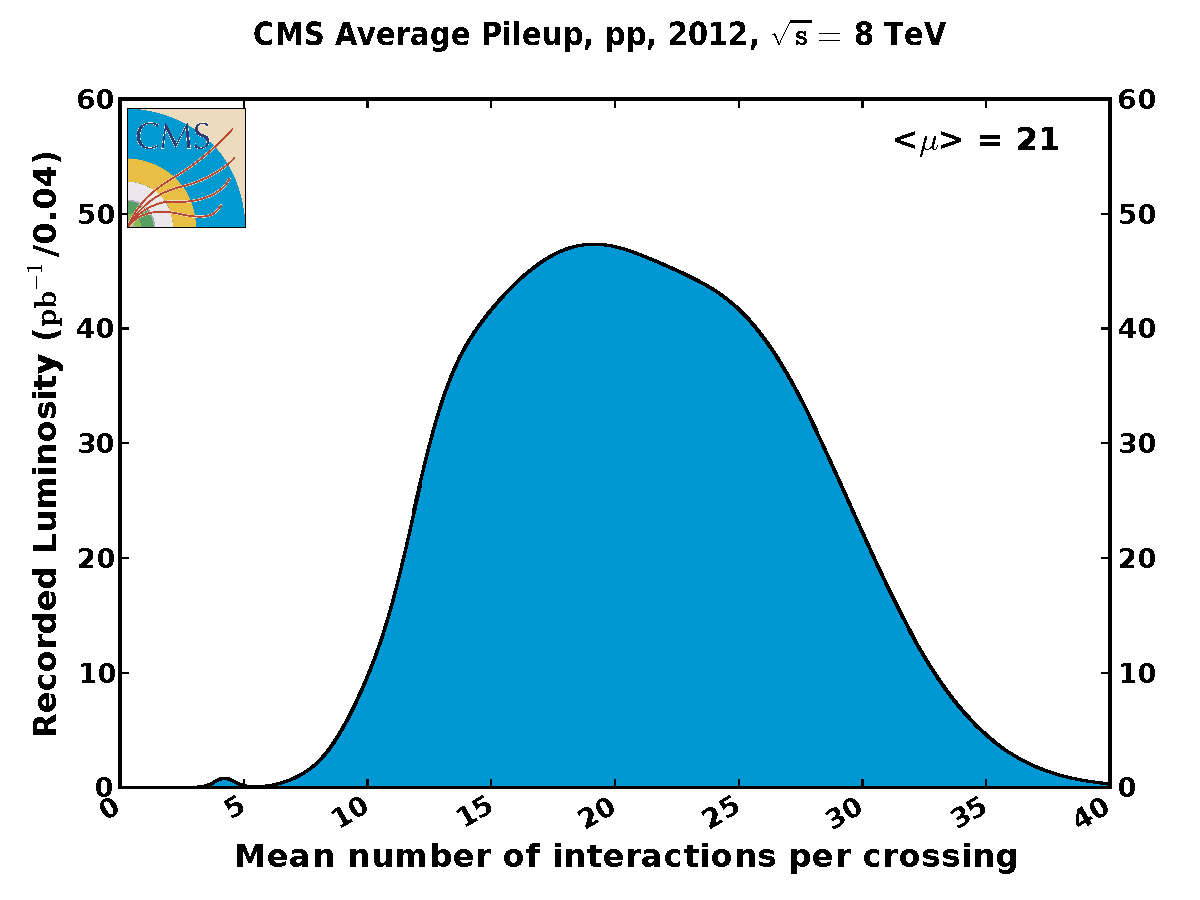
\includegraphics[width=1.2\largefigwidth]{plots/detector/pileup_pp_2012.pdf}
  \caption{Distribution of the number of interactions per bunch crossing in CMS during 2012 running of the LHC.\cite{CMSLumiPublic}}
  \label{fig:pusummary}
\end{figure}


\section{The \CMS experiment}
\label{sec:CMSInDetail}
%??Introduction - describe hermetic onion shell concept and introduce subsystems
The CMS detector was designed to search for the SM Higgs and new physics at the TeV energy scale. Both because the nature of new physics is not known and the SM Higgs has a wide range of decays and production mechanisms CMS must be sensitive to many different types of final state particles and topologies. In order to achieve this it has a hermetic design comprising a barrel, endcaps and a forward calorimetry system, and is also composed of several layers of subdetectors each sensitive to different particles as shown in \FigureRef{fig:cmsschematic1}. The hermiticity of the detector is particularly important for the VBF Higgs to invisible search, because, as described in \SectionRef{sec:higprod}, the VBF final state is highly likely to have jets in the forward regions of the detector.

A central design feature of CMS is the superconducting magnet, inside which is generated a 3.8T axial field. This field bends the path of charged particles travelling through it allowing their momentum to be measured. Not all particles are charged however, and the path of several types of particles through the CMS detector is shown in \FigureRef{fig:cmsschematic2}. The first layer is the tracker which records the paths taken by charged particles, as well as providing a momentum measurement the tracks also allow the vertex the particle came from to be identified. The next layer is the \ac{ECAL} where electrons and photons deposit energy through electromagnetic showers. This is followed by the \ac{HCAL} where hadronic showers deposit most of their energy. After the calorimetry systems is the superconducting magnet which is not instrumented. Outside the magnet are the muon detection systems, which are interspersed with iron plates which form the return yoke for the magnet. Muons do not deposit much energy in the detector and often are not stopped, so the muon system is primarily a tracking detector.

%??Coordinate system
The origin of the co-ordinate system used by CMS is at the nominal interaction point. It is a right handed cartesian system with the x axis pointing towards the centre of the LHC ring and the y-axis vertically upwards, the z axis then points along the beam line. The azimuthal angle $\phi$ and the polar angle $\theta$ are measured from the x and z axes respectively. It is common to describe the direction of outgoing particles using $\phi$ and their pseudo-rapidity, $\eta$ which is defined as:
\begin{equation}
  \label{eq:eta}
  \eta=-\ln[\tan(\theta/2)].
\end{equation}
Distances in the $\eta-\phi$ plane are given by $\Delta R=\sqrt{\Delta\phi^2+\Delta\eta^2}$. Two other important quantities in hadron colliders are the projections of a particle's momentum and energy in the transverse plane, these are denoted \pt and \Et respectively.

\begin{figure}
  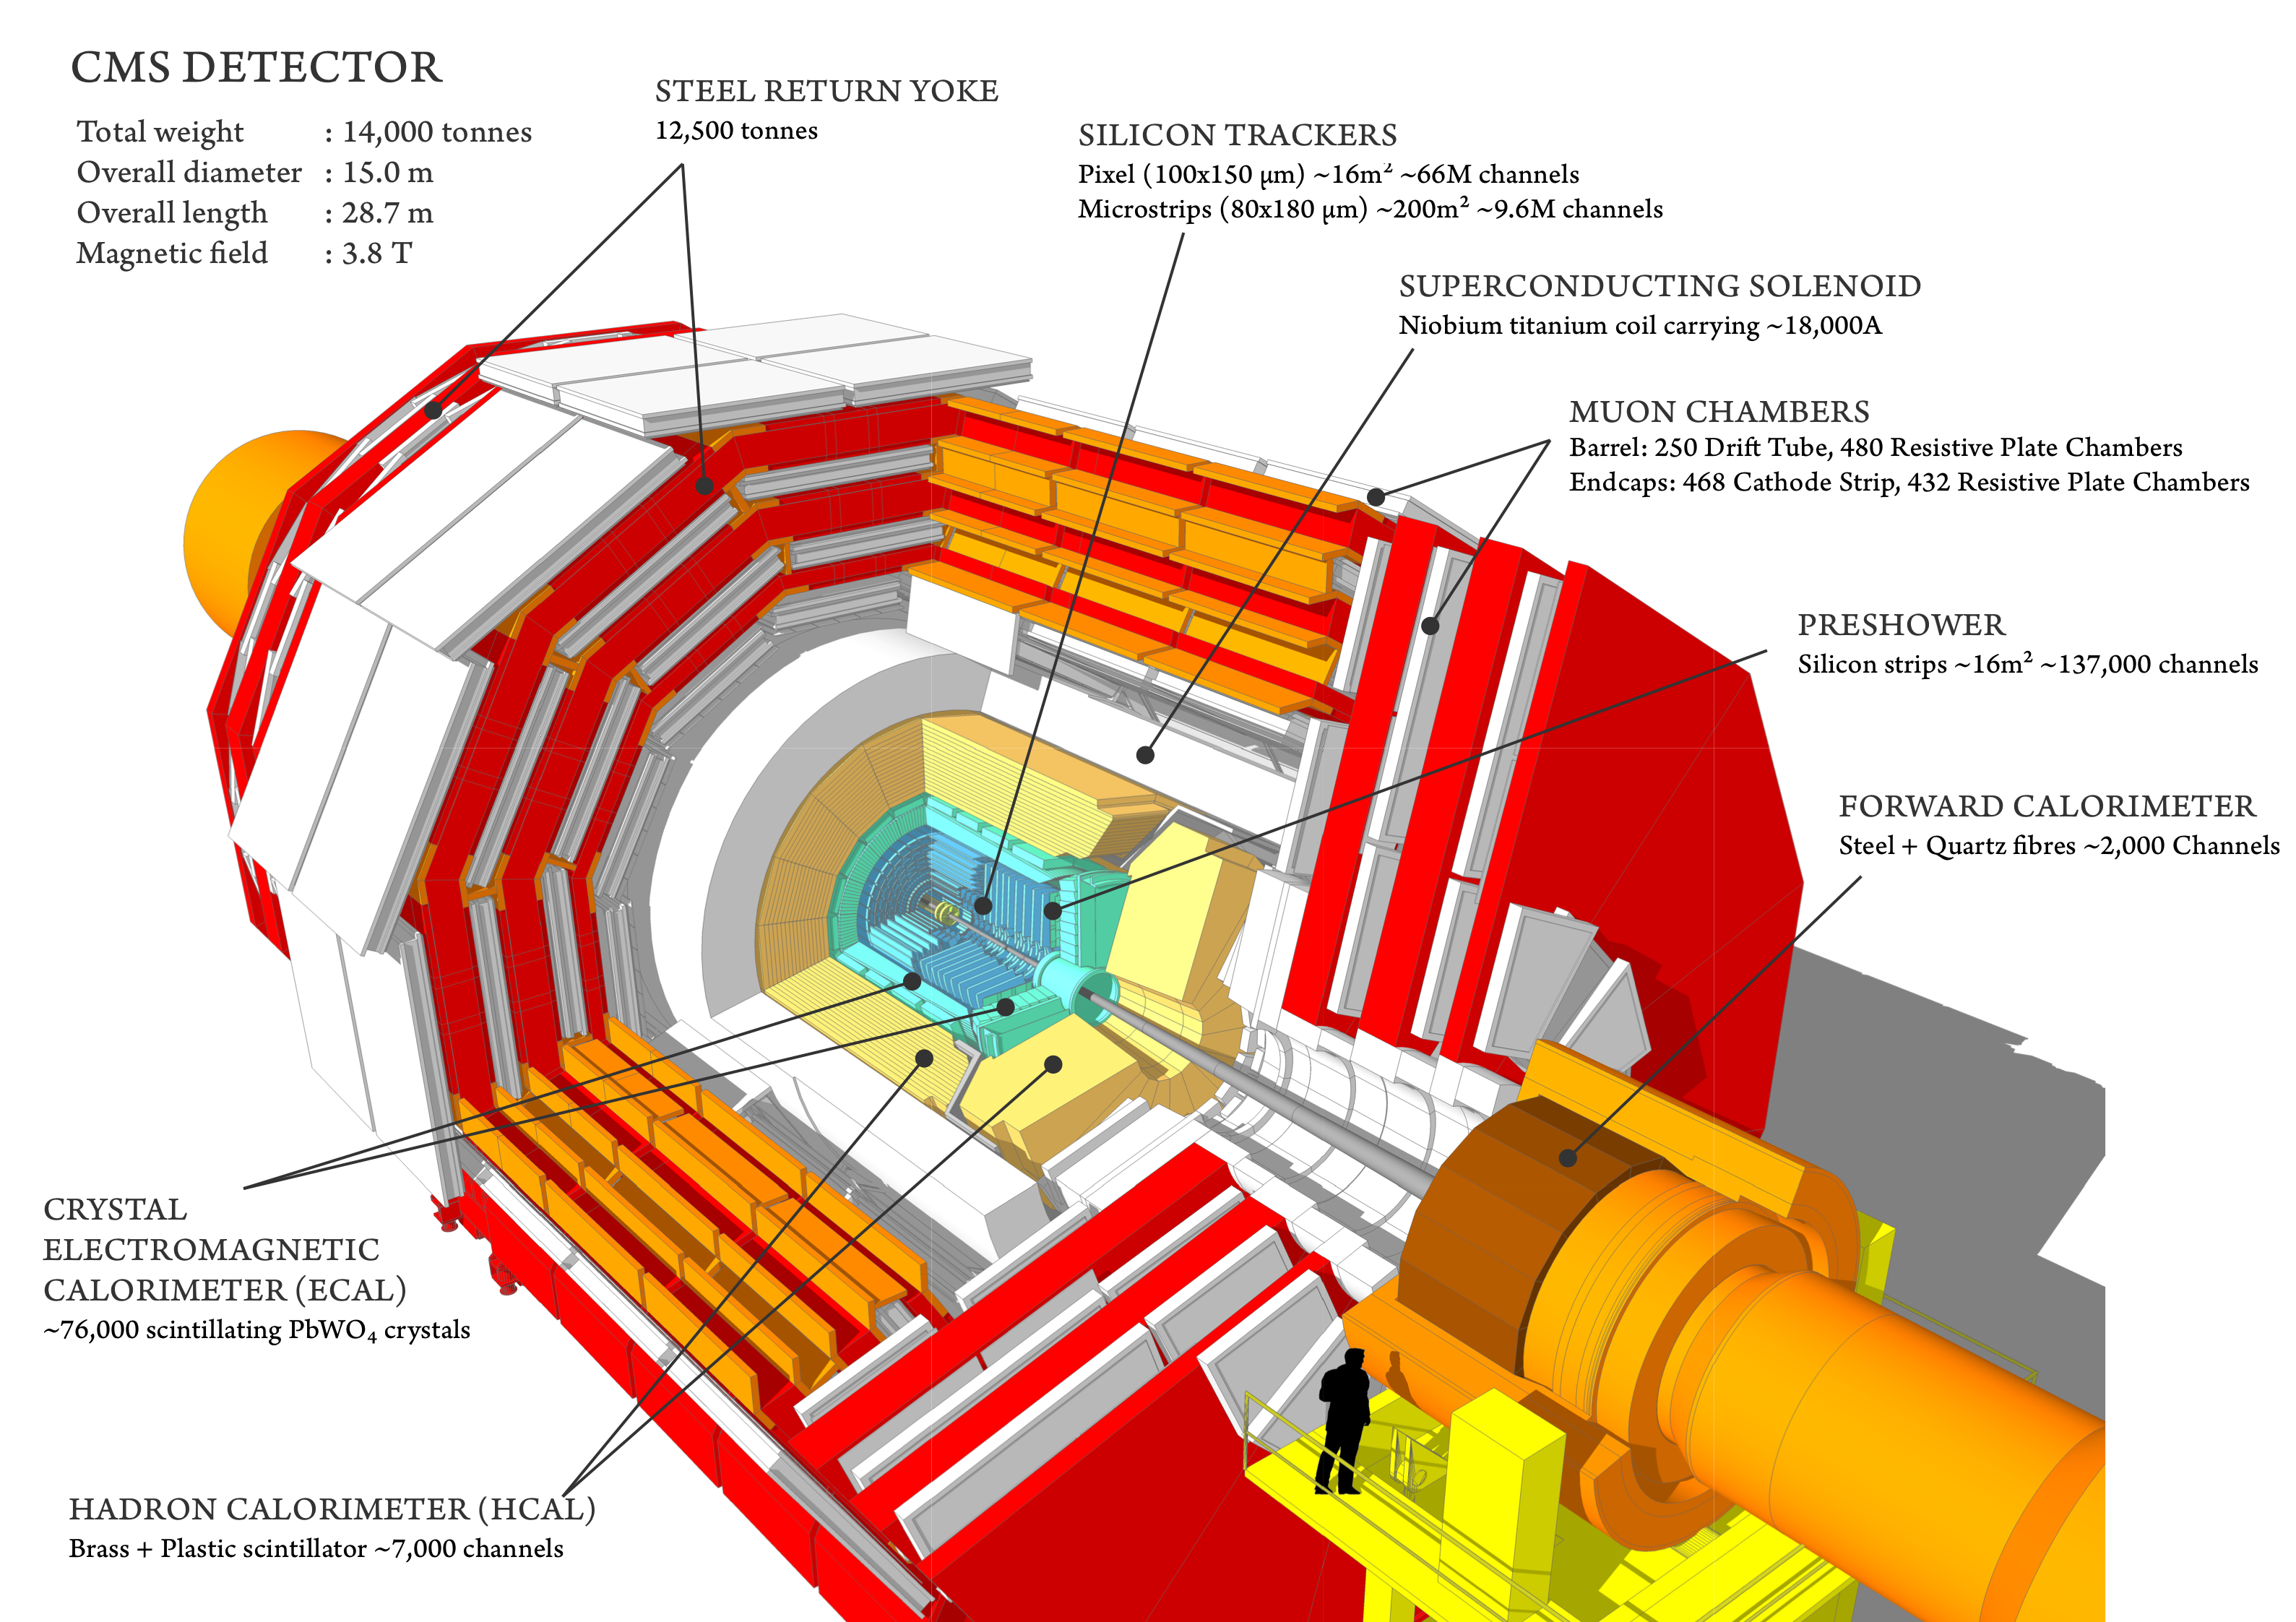
\includegraphics[width=1.2\largefigwidth]{plots/detector/cms_120918_03.png}
  \caption{A diagram of the subsystems making up the CMS detector, illustrating the hermeticity and layered structure of the experiment.\cite{cmsschematic}}
  \label{fig:cmsschematic1}
\end{figure}

\begin{figure}
  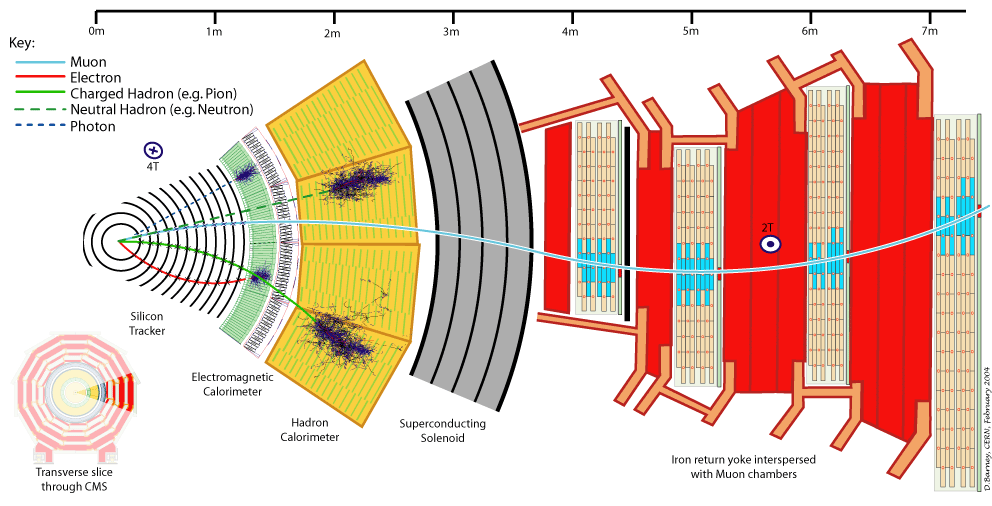
\includegraphics[width=1.2\largefigwidth]{plots/detector/CMS_Slice.png}
  \caption{A schematic cross-section of the CMS experiment showing the path taken by several types of particles.\cite{CMSSlice}}
  \label{fig:cmsschematic2}
\end{figure}

\subsection{Tracker}
\label{sec:tracker}
%??Describe Tracker
The tracker is designed to precisely measure the paths of charged particles coming from LHC collisions, this allows the particles' momentum along with the position of the vertex that they came from to be determined. In order to precisely measure the particles' positions high granularity is required. Additionally, due to the frequency of collsions at the LHC and the high instantaneous luminosity a radiation hard system with fast response is also necessary. This combination of requirements motivates the use of a silicon based system \cite{Chatrchyan:2008aa}.

%??Submodules
The tracker layout can be seen in \FigureRef{fig:trackerschematic}. It is made up of a pixel detector which has three layers in the barrel and two in the endcap, and a strip detector with 10 layers in the barrel and 9 layers in the endcap. The barrel and endcap detectors together have an acceptance of $|\eta|<2.5$.
%??Resolution

\begin{figure}
  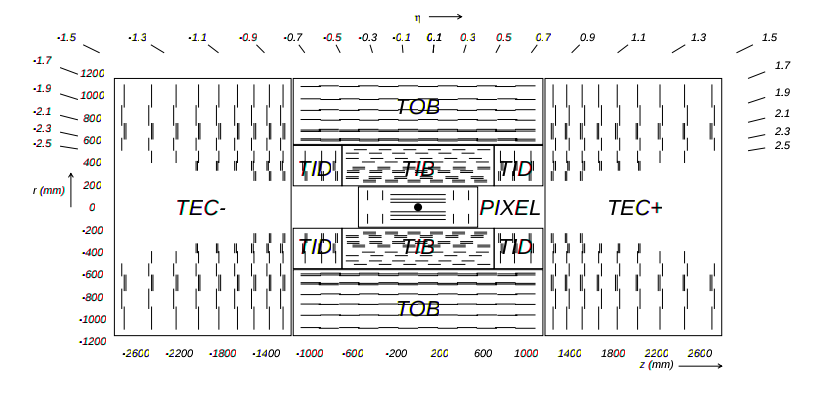
\includegraphics[width=1.2\largefigwidth]{plots/detector/TrackerSchematic.png}
  \caption{A cross-section of the CMS tracker, indicating the subsystems that comprise it. Each line indicates a detector module \cite{Chatrchyan:2008aa}.}
  \label{fig:trackerschematic}
\end{figure}

\subsection{Electromagnetic calorimeter}
\label{sec:ECAL}
%??Describe ECAL
%??Submodules
%??Resolution

\subsection{Hadronic calorimeter}
\label{sec:HCAL}
%??Describe HCAL
%??Submodules
%??Resolution

\subsection{Muon system}
%??Describe muon system
%??Submodules
%??Resolution

\subsection{Trigger system}
\label{sec:triggers}
%??Describe trigger system

